\section{Alternative auxiliary-circle proofs of the inverse problem}
\label{sec:alternative-proof}

In this section we give more derivations of the same $1/r^2$ law, still using the auxiliary circle $C$ (center $O$, radius $a$), but emphasizing a different set of local ellipse facts so that the argument has as few moving parts as possible. Similar to Newton's methods, these approaches apply to other forms of conic sections as well, and we will discuss this further in \Cref{sec:other-conics}.

\begin{figure}[t]
  \centering
  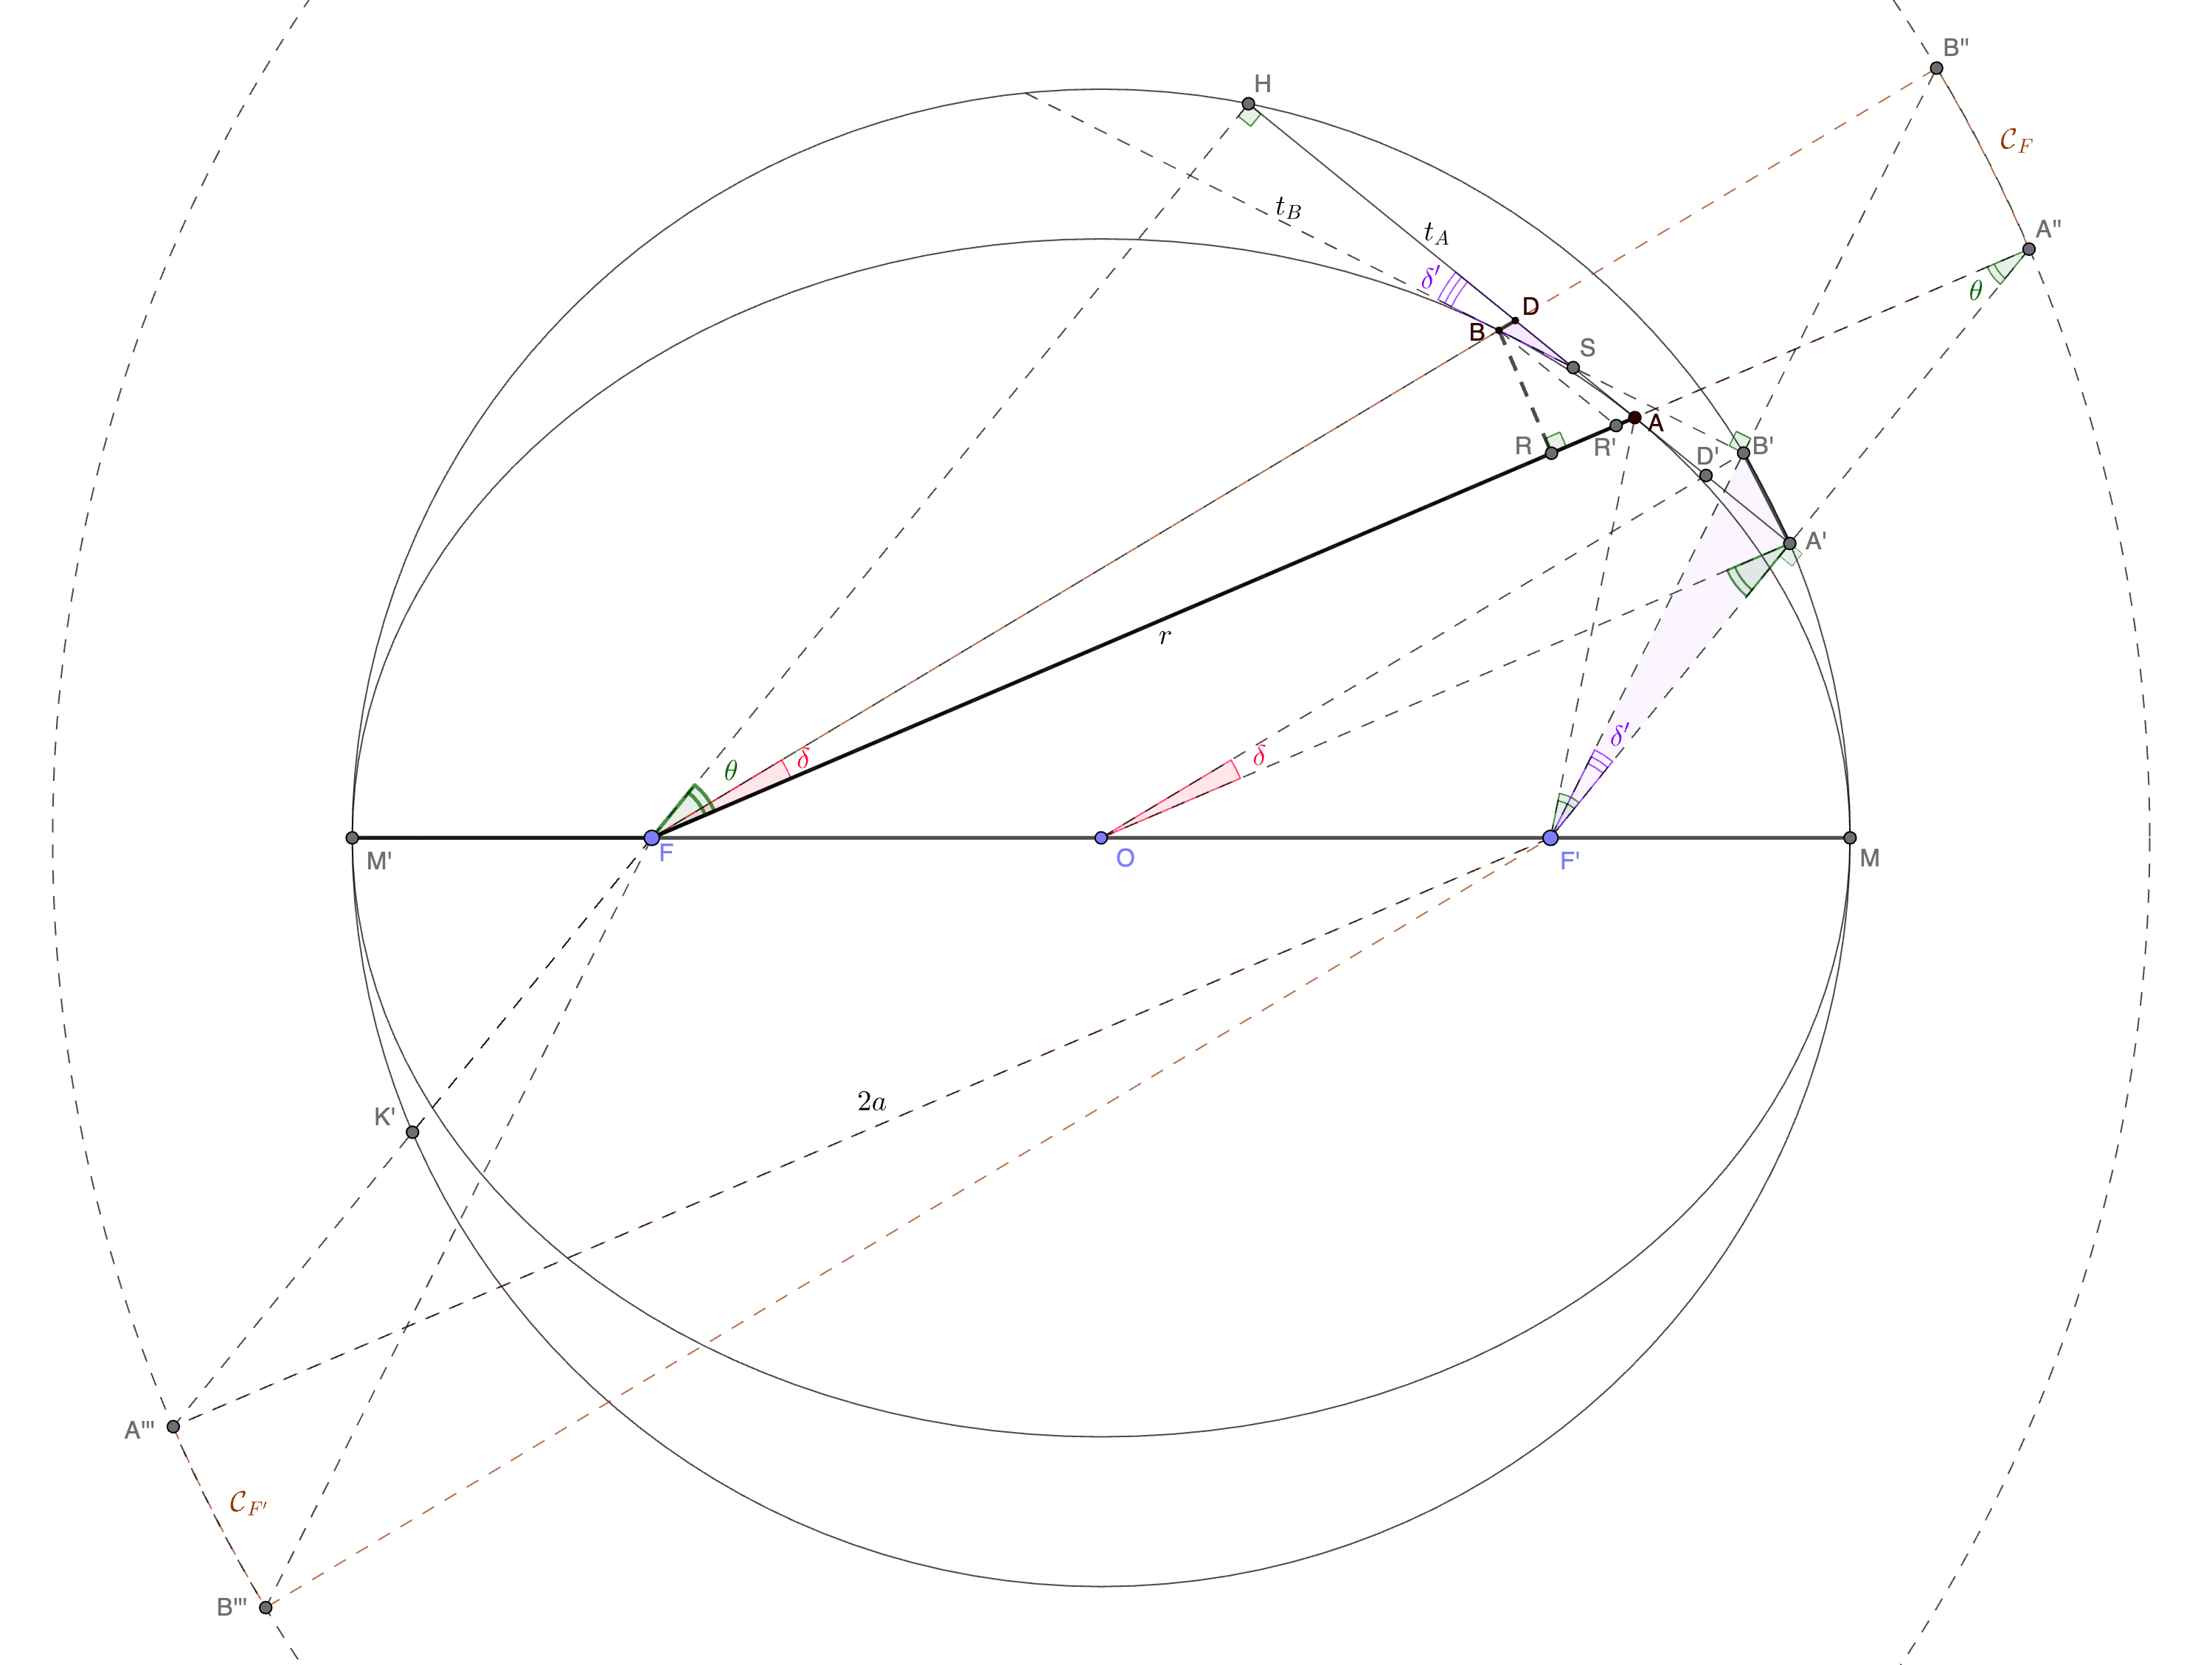
\includegraphics[width=\linewidth]{assets/images/ellipse_proof2_with_directrix.png}
  \caption{Alternative auxiliary-circle construction used in Section~\ref{sec:alternative-proof}.The angles $\delta$ and $\delta'$ are approaching 0 as $B\to A$. The directrix circles $\mathcal{C}_F$ and $\mathcal{C}_{F'}$ are shown for reference; they are not used in the proof but can replace the auxiliary circle as alternatives. All three circles are also alternative rotated hodographs as metnioned in \Cref{sec:forward-problem-hodograph}.}
  \label{fig:proof2-ellipse}
\end{figure}

\subsection{Geometric setup}

Let the ellipse have foci $F,F'$. Fix a point $A$ on the ellipse and write $r=FA$.
Let the tangent at $A$ meet the auxiliary circle again at $A'$. For a nearby point $B$ on the ellipse, let its tangent meet the same auxiliary circle at $B'$. We let $B\to A$.
Denote these tangent lines by $t_A$ and $t_B$, respectively; the instantaneous velocity vectors $\mathbf v_A$ and $\mathbf v_B$ are directed along $t_A$ and $t_B$.

Let $D$ be the intersection point on the tangent construction (as in \Cref{fig:proof2-ellipse}), and let $R$ be the foot used to form the small segment $BR$ (the small transverse piece in the right triangle at $R$).

\begin{lemma}[Product identity]
  \label[lemma]{lem:product-identity}
  With the notation of \Cref{fig:proof2-ellipse},
  \begin{equation}
    FH\cdot F'\!A'=(a-c)(a+c)=b^2,
  \end{equation}
  where $c=OF$ is the focal distance (so $a^2=b^2+c^2$).
\end{lemma}

\begin{proof}
  Since $FK' \parallel F'A'$ in the construction, triangles with corresponding sides along these parallels are similar, and the segment on the parallel through $F$ has the same length as the corresponding segment on the tangent through $F'$. In particular,
  \begin{equation}
    F'\!A' = FK'.
  \end{equation}
  Therefore
  \begin{equation}
    FH\cdot F'\!A' = FH\cdot FK' = (a-c)(a+c)=a^2-c^2=b^2,
  \end{equation}
  which is the standard ellipse identity.
\end{proof}


\subsection{Iverse problem Proof 2 of the ellipse case}

\begin{proof}
As $B\to A$, the little segments cut off by nearby tangents/secants agree to first order; thus the similar-triangle relations used below are valid in the Newtonian (1687) ``ultimate ratio'' sense (any error is higher order and vanishes in the limit).

Similarity in \Cref{fig:proof2-ellipse} gives
\begin{equation}
  \triangle SDB \sim \triangle F'\!A'B'
  \qquad\Longrightarrow\qquad
  BD=SD\cdot\frac{A'B'}{A'F'}.
\end{equation}
By \Cref{lem:deflection-identity} in Section~\ref{subsec:central-direction-lemmas}, $SD=\frac12\,AD$, hence
\begin{equation}
  BD=\frac12\,AD\cdot\frac{A'B'}{A'F'}.
\end{equation}

From focal-geometry and auxiliary-circle similarities (equivalently, affine scaling ellipse $\leftrightarrow$ circle),
\begin{equation}
  \begin{aligned}
    AD&=\frac{AF}{FH}\,BR=\frac{r}{FH}\,BR,\\
    A'B'&=\frac{OA'}{F'\!A}\,BR=\frac{a}{r}\,BR.
  \end{aligned}
\end{equation}
\begin{equation}
  BD=\frac12\left(\frac{r}{FH}BR\right)\left(\frac{a}{r}BR\right)\frac{1}{A'F'}
  =\frac12\,a\,\frac{BR^2}{FH\cdot A'F'}.
\end{equation}
By \Cref{lem:product-identity}, $FH\cdot A'F'=b^2$, hence
\begin{equation}
  BD=\frac12\,a\,\frac{BR^2}{b^2}.
\end{equation}
Using $p=b^2/a$,
\begin{equation}
  BD=\frac{1}{2p}\,BR^2,
  \label{eq:proof2-bd-br2}
\end{equation}
so
\[
  \frac{BD}{BR^2}\to \frac{1}{2p}.
\]
Applying \Cref{lem:bd-over-br2} with $\kappa=\frac{1}{2p}$ gives immediately
\[
  a_F=\frac{2\kappa L^2}{r^2}=\frac{L^2}{p}\frac{1}{r^2},
  \qquad
  \mathbf a_F(r)=-\mu\,\frac{\mathbf r}{r^3},
  \qquad
  \text{i.e. }\mathbf a_F(r)=-\frac{\mu}{r^2}\,\hat r,
  \qquad
  \mu=2\kappa L^2=\frac{L^2}{p}.
\]
\end{proof}

\subsection{Inverse problem Proof 3 (hodograph-style computation)}
\label{subsec:proof3-hodograph}

From \Cref{lem:product-identity},
\begin{equation}
  F'\!A'=\frac{b^2}{FH}.
\end{equation}
Let $v=\lvert \mathbf v\rvert$ be the speed at $A$. Since the velocity direction is tangent to the orbit and $FH$ is perpendicular to that tangent (as in the construction), the areal-rate constant gives
\begin{equation}
  FH\cdot v = L.
\end{equation}
Combining,
\begin{equation}
  F'\!A'=\frac{b^2}{FH}=\frac{v\,b^2}{L}.
\end{equation}
For two nearby points $A,B$ we therefore have, in the Newtonian small-step sense,
\begin{equation}
  A'B'=\Delta(F'\!A')=\frac{b^2}{L}\,\Delta v
  =\frac{b^2}{L}\,a_F\,\Delta t,
\end{equation}
where $a_F$ is the magnitude of the (focus-directed) acceleration and we used \Cref{lem:deflection-identity} ($\Delta v=a_F\Delta t$).
On the other hand, from the auxiliary-circle similarity used above,
\begin{equation}
  A'B'=\frac{OA'}{F'\!A}\,BR=\frac{a}{r}\,BR.
\end{equation}
Eliminating $A'B'$ gives
\begin{equation}
  a_F=\frac{L}{b^2}\,\frac{A'B'}{\Delta t}.
\label{eq:proof3-af-from-ab}
\end{equation}
Next, using again the auxiliary-circle similarity $A'B'=\frac{a}{r}BR$ and \Cref{lem:bd-over-br2} ($BR\sim L\Delta t/r$), we have
\begin{equation}
  A'B'=\frac{a}{r}\,\frac{L\,\Delta t}{r}
  =\frac{a}{r^2}\,L\,\Delta t.
\label{eq:proof3-ab-from-br}
\end{equation}
Combining \eqref{eq:proof3-af-from-ab} and \eqref{eq:proof3-ab-from-br} yields
\begin{equation}
  a_F=\frac{L^2}{p}\,\frac{1}{r^2},
  \qquad
  \mathbf a_F(r)=-\mu\,\frac{\mathbf r}{r^3},
  \qquad
  \text{i.e. }\mathbf a_F(r)=-\frac{\mu}{r^2}\,\hat r,
  \qquad
  \mu=\frac{L^2}{p}.
\end{equation}
exactly the same inverse-square formula as in \Cref{prop:proof1-ellipse-inverse-square}.
\hfill$\square$

\subsection{Discussion: directrix circle and a hodograph viewpoint}
\label{subsec:sec6-discussion}

\paragraph{Directrix circle variant.}
One can re-run essentially the same similarity argument by replacing the auxiliary circle $\mathcal C$ (center $O$, radius $a$) with the \emph{directrix circle} centered at $F$ of radius $2a$ (cf.\ the construction used in Section~3).
Extending $FA$ to meet this directrix circle at $A''$, one has $A''A'F'$ colinear; similarly, extending $FB$ meets the directrix circle at $B''$ with $B''B'F'$ colinear.
Moreover, $A'$ and $B'$ are midpoints of the segments $A''F'$ and $B''F'$, respectively, so
\begin{equation}
  A''B'' = 2\,A'B'.
\end{equation}
Consequently,
\begin{equation}
  \triangle A'B'F' \sim \triangle A''B''F',
\end{equation}
and the same chain of similar-triangle identities yields the same ultimate-ratio estimate for the normal drop $BD$, hence the same inverse-square dependence.

\paragraph{Connection to Maxwell's hodograph.}
The product identity in \Cref{lem:product-identity} (already implicit in classical ellipse geometry) also appears in Maxwell's 1877 discussion of the \emph{hodograph} of planetary motion: for an inverse-square central force the velocity vector $\mathbf v(t)$ traces a circle in velocity space (Hamilton's 1847 hodograph), and Maxwell notes that this hodograph circle is similar to the directrix circle, with its ``speed origin'' at $F'$, but rotated by $90^\circ$ counterclockwise \cite{maxwell1877mattermotion}.

From this point of view, our construction may be read as relating the geometric drop $BD$ directly to a rotated hodograph circle $C$.
This suggests that the previous Proof 3 is essentially a repetition of Maxwell's approach to the inverse problem, but with the auxiliary circle $\mathcal{C}$ playing the role of the hodograph circle instead of the directrix circle. All three circles are alternative rotated hodographs for the same inverse-square dynamics, and any of them can be used in a similar way to relate the geometric drop $BD$ to the velocity change $\Delta v$. Moreover, the same auxiliary-cicle can also have two different interpretations treating either F or F' as the velocity origin, this is by noting that K' as the image of A' under the symmetry about center O. As argued in \cite{carinena2016newlook}, argued the two directrix circles can both be viewed as the transformed hodograph with either force F as the origin or F' as the origin; and circle $\mathcal{C}_F'$F being the rotated hodograph around focus F has additional advantage with the common polar origin. In the auxiliary-circle construction, either directrix circle is simply a scaled version of the auxiliary circle with the scale center being either F or F'.
